\chapter{Design}
After analyzing the problem, this chapter will go through the design of the application architecture of our UIProtocol client. The design phase is of crucial importance as it is the time when important design decisions are made. In this phase, the application's architecture needs to be thought through so that its future extensions are relatively easy to implement and cost of maintenance is low.\\
From the analysis we will conclude requirements for the application which will be developed. Further on, the sections will describe the design of several sub-systems which are responsible for handling the communication, models, events, inner representation of the UI elements, their rendering and more.\\
Even though there are existing implementations of UIProtocol client, the design of this one was not influenced by any of them.

\subsection{Requirements}
The client application will be developed and run on Windows Phone 8 device. Since the entire user interfaces and information about events is intended to be transferred over wireless internet connection, there will be a delay present in the application's reaction time, which is a inescapable consequence of the client-server architecture. The delay should be reasonably small to allow for a comfortable usage of the application. Even with this delay, the application should perform well in terms of UI rendering times, reaction time and overall feel.\\
There is a number of requirements an app should meet in order to be truly accessible. In our analysis, we found that the support of Windows Phone 8 for accessibility is lower than at the competing platforms. Namely, support for a key accessibility feature, a screen reader, is not present by default. This holds true even for the Windows Phone 8.1 which was released in February 2014. This can be a major flaw to the application accessibility – especially for visually impaired who would have to use a third-party screen reader in order to be able to navigate through the app. Apart from following the guidelines for developing accessible apps, as discussed in \ref{sec:accGuidelines}, we may propose some new features that could be implemented by UIProtocol to increase its own support for accessibility. At any rate, even with the Windows Phone 8 platform's low accessibility support, the developed app will remain a fully functional UIP client capable of displaying valid UIP documents.


\subsubsection{Summary of Requirement}
From the requirements section, we have developed the following lists of non-functional and functional requirements, respectively.
\\
Non-functional requirements:
\begin{itemize}
  \item UI components have platform native look
  \item App will be will be written in C\#
  \item The client should not use much phone resources when idle
  \item App should be stable and able to process valid UIP documents
  \item Compatibility with UIP standard, draft 8
  \item Ability to run on any WP8 device
  \item UI loading times below 0.5 s with stable internet connections
\end{itemize}
~\\
Functional requirements:
\begin{itemize}
  \item  Support for basic user interface elements
  \item Graceful degradation for unsupported elements
  \item  Support for binding and model-wide binding
  \item  Support for interpolated model updates (animations)
  \item  Support for UI generator API
  \item Support for absolute and grid layouts
  \item Support for styling (font size, colors, etc.)
\end{itemize}

\subsection{Client-server Communication}
The client will communicate with the server over TCP-IP connection which will be handled by a standard socket. Upon this communication channel, UIProtocol XML files will be transferred.\\
Once the client connects to the server and goes through the connection procedure described in \cite{uip}, the server sends the XML files describing the UI. The UML diagram of the classes responsible for the communication is shown in figure \ref{fig:classComm}.

\begin{figure}[ht!]
\centering
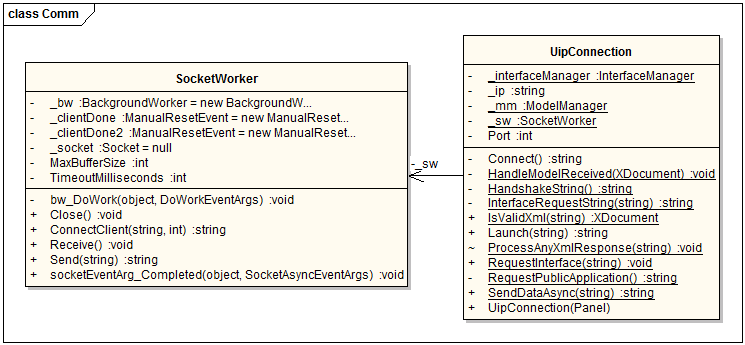
\includegraphics[width=145mm]{pics/3/classComm.png}
\caption{Inheritance tree of several sample UI classes}
\label{fig:classComm}
\end{figure}

\subsection{Parsing XML into Inner Object Representation}
When the UIP documents are received, they will be delegated to instances of ModelManager and InterfaceManager classes. ModelManager will be responsible for processing possible new models or model updates and will be discussed later.\\
The InterfaceManager class will process the XML data that describes the UI by recursively traversing the XML tree and creating instances of Interface, Container and Element classes, based on the type of the considered XML node.

\begin{figure}[ht!]
\centering
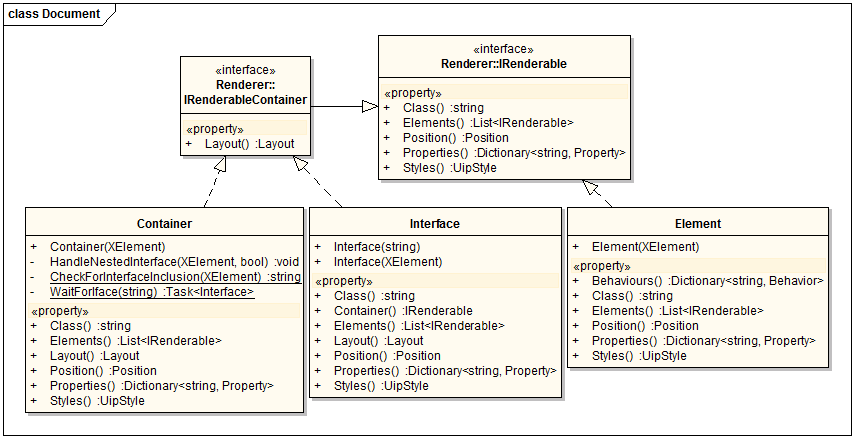
\includegraphics[width=145mm]{pics/3/classDocument.png}
\caption{document class diagram}
\label{fig:classDocument}
\end{figure}

\subsection{Managing Models}
If an UI element has a property that refers to a model, ModelManager will be responsible for requesting the model containing the property. Once it is received, it will be processed by the ModelManager instance which will keep their value stored and will manage future model updates.


\subsection{Managing Interfaces}

\subsection{Rendering the UI}
After the XML description of UI elements is processed, rendering takes place. The Renderer class traverses the tree of the newly created classes from figure todo and calls the 
\\behavior, leyouts, positions, tcp and uipconnection, settings

\subsection{Representing the Platform-native UI Components}
In order to support easy addition of the supported UI elements, we created classes shown in figure todo. There is an abstract base class, UipBase which contains methods for model updates, styling and element dimensions.\\
Any particular UI element needs to inherit from the base class in order to support rendering, model updates and other functionality provided by the base class.

\subsection{Events}
Events are triggered by user actions - usually clicking on an interactive UI element such as button. The event firing - e.g. notifying server of an action taking place, is a relatively simple process which will be handled by two classes: EventManager: the class's only task is to provide a method for sending an event. The class won't contain any state and will therefore be static, and will only forward the events to SocketWorker class instance. 
Event class will represent a particular event that will be sent to the server. It will contain all the necessary information for the server to be able to identify the event triggered.

\begin{figure}[ht!]
\centering
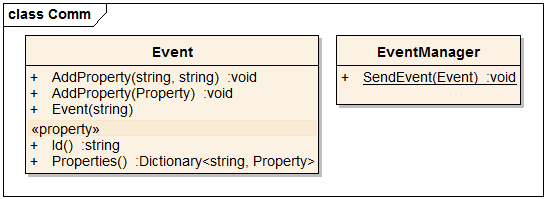
\includegraphics[width=130mm]{pics/3/classEvent.png}
\caption{event class diagram}
\label{fig:classEvent}
\end{figure}

\subsection{Properties}
Properties are the most nested objects in UIP documents. They are used extensively within many classes, including Model, Event or Element. They are directly attached to the class instance.

\begin{figure}[ht!]
\centering
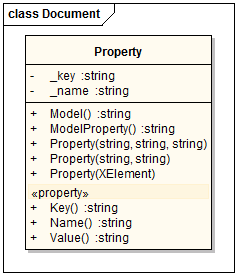
\includegraphics[width=60mm]{pics/3/classProperty.png}
\caption{properties class diagram}
\label{fig:classProperty}
\end{figure}

